\subsection{PTF best practices: the basics }
In this section we will walk through the basics of how best to approach the instrumentation and tuning of applications with PTF in the context of an example application.

To begin our walk-through demonstration on how to best exploit PTF, we first choose to work with the BT-MZ benchmark. The BT benchmark is part of the NPB (NASA Parallel Benchmark) Suite \cite{NPB} and contains the kernel for a Block Tri-diagonal solver. BT-MZ is a multi-zone version of the BT benchmark which is designed to exploit multiple levels of parallelism in the application. The BT-MZ application is written in FORTRAN with over 4.5k lines of code. The application is a serial application running on a single core, where there is a potential for performance optimization through using a combination of various compiler flags. As an application developer, we typically have some idea of the compiler flags that are important for performance improvements but not necessarily the optimal combination of the these flags. We also know that the incorrect combination of flags may actually degrade the performance of our application. The required manual experimentation of different flag combinations can be time consuming and cumbersome, so we would like a tool to automate the task of selecting the optimal combination of the compiler flags. The Compiler Flags Selection (CFS) plugin from PTF does exactly this and also provides some additional features, which we will walk through in the following sections.

\subsubsection{Building the application with the PTF plugin}

Using information in the CFS Plugin User's Guide \cite{CFSguide} the BT-MZ benchmark application is compiled.
From the CFS Plugin User's Guide we learn that instrumentation of the application is required so that PTF can collect performance measurements. In order to collect measurements, the compilation process is tweaked to use the \texttt{psc\_instrument} command to perform instrumentation while compiling the application, as shown in Figure~\ref{fig:uc1_CFS_make_file}.

\begin{figure}[H]
	\centering
	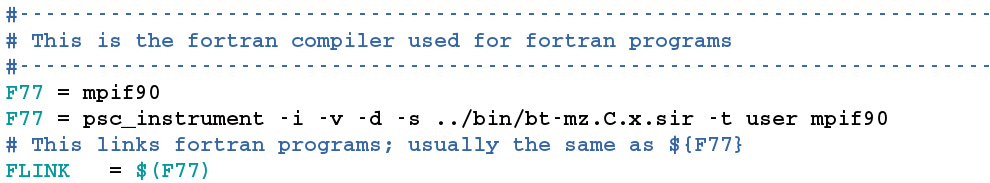
\includegraphics[height=3cm, width=\textwidth]{../BPG/images/uc1_CFS_make_file.png}
	\caption{Change made to make.def file to add {\tt psc\_instrument} wrapper }
	\label{fig:uc1_CFS_make_file}
\end{figure}

In order to test each possible combination of compiler flags, PTF recompiles the application with each combination. PTF is informed about the compilation steps and arguments using the cfs\_config.cfg file, as mentioned in the CFS Plugin User's Guide (available on the PTF website). A template for the configuration file is installed along with the PTF installation. A configuration file used for this example can be seen in Figure \ref{fig:uc1_cfs_config}.

\begin{figure}[H]
	\centering
	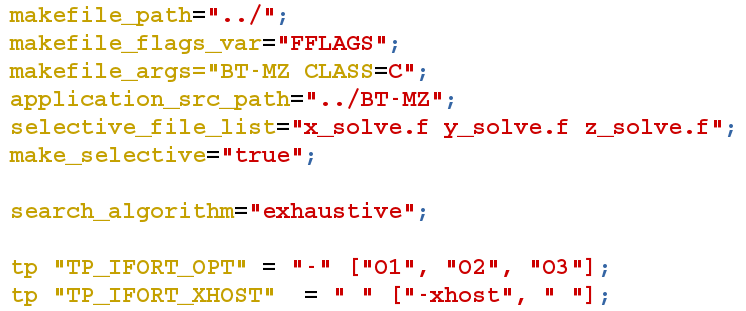
\includegraphics[scale=0.65]{../BPG/images/uc1_cfs_config.png}
	\caption{An example of a configuration file for the CFS plugin.}
	\label{fig:uc1_cfs_config}
\end{figure}


\subsubsection{Running the application with PTF for the first time}
Subsequent to this build step, the BT-MZ application is executed using the PTF {\tt psc\_frontend} command as shown in the PTF User's Guide \cite{PTFguide}. After successful execution, the optimal combination of compiler flags along with a summary of results for each combination is reported by the CFS plugin. For the example that we provide here, the search for the optimal combination of flags took approximately 4697 seconds. This overhead is expected because running PTF for this basic example involves recompilation and re-execution of the application with each combination of the selected compiler flags. Sample output of the PTF execution for the BT-MZ example discussed here is shown in Figure \ref{fig:uc1_cfs_output}.

\begin{figure}[H]
	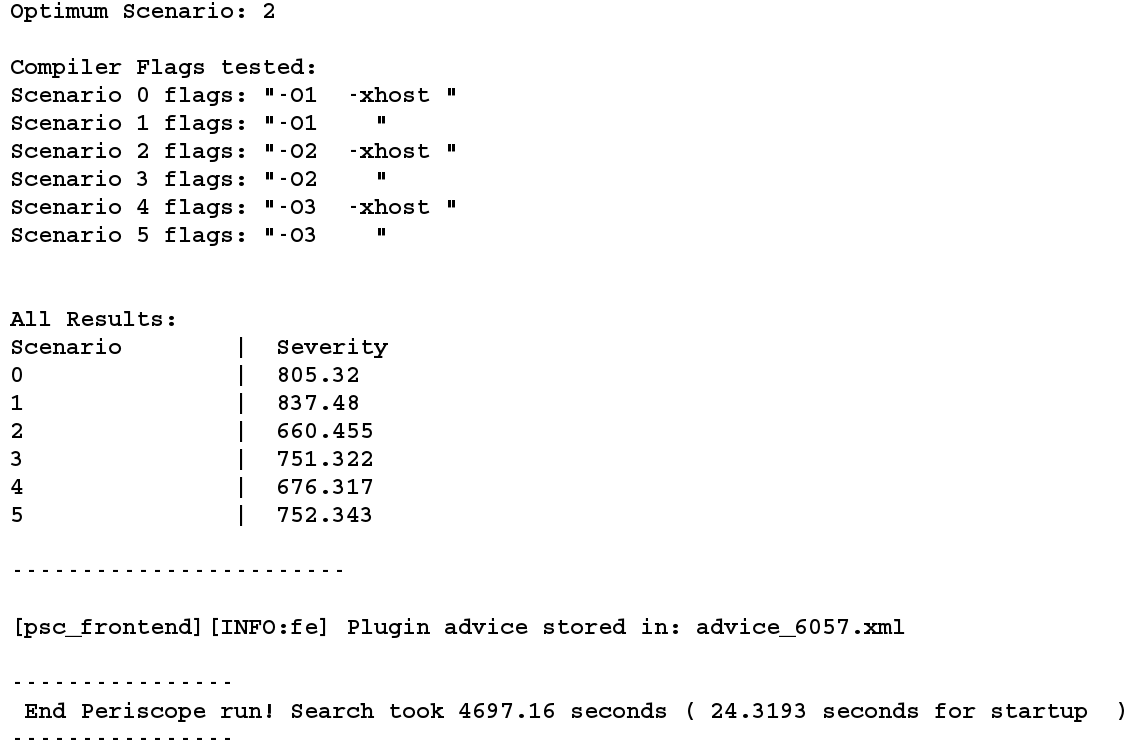
\includegraphics[width=\textwidth]{../BPG/images/uc1_cfs_output.png}
	\caption{Sample output of PTF execution for the BT-MZ benchmark in naive mode.}
	\label{fig:uc1_cfs_output}
\end{figure}

\subsubsection{Reducing the overall execution time using a phase region}

The PTF User's Guide explains the concept of a \emph{phase region}. Many HPC applications have a global progress loop, e.g., going through the simulated time steps. The execution of the loop body for a single time step is called a phase. The phase region, i.e., the loop body, can be marked for PTF in the source code as a \emph{user region}. If the phase region is given, PTF will perform all experiments for a single iteration instead of executing the entire loop and thus, significantly reducing the tuning time. If no phase region is marked via a user region, the main program region is used as the default phase region. 

In our example, BT-MZ has a main time-stepping loop with a trip count of 200, where the same type and amount of computation was executed for each iteration of the loop.  A PTF user region can therefore be placed around the body of this computationally dominant loop. Only two pragma lines are required to be inserted into the BT-MZ source code, representing the start and end of the user region, respectively. For the BT-MZ example, this results in PTF executing only one iteration of the time-stepping loop rather than the full 200 iterations, reducing the execution time of PTF to approximately 227 seconds (relative to 4697 seconds without User Regions). Sample output from a PTF run using the phase region approach is shown in Figure \ref{fig:uc1_user_regions}.

\begin{figure}[H]
	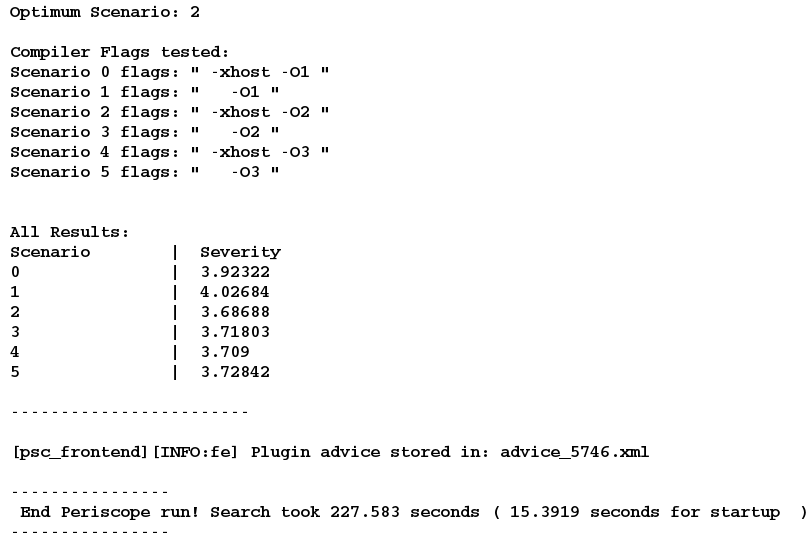
\includegraphics[width=\textwidth]{../BPG/images/uc1_user_regions.png}
	\caption{CFS output for the BT-MZ application with a marked phase region and selective make enabled.}
	\label{fig:uc1_user_regions}
\end{figure}

\subsubsection{Reducing initialization time}
The PTF User's Guide provides information on the ``fast starter'' flag which can reduce the amount of time spent in the initialization of PTF. For example, by passing {\tt --starter=FastInteractive} to the {\tt psc\_frontend} command,  the total execution time for PTF can be reduced further to approximately 161 seconds for the BT-MZ example described here (reducing the time spent in initialization time from approximately 20 seconds to 5 seconds. Sample output showing the effect of {\tt --starter=FastInteractive} can be seen in Figure \ref{fig:uc1_fast_interactive}.

\begin{figure}[H]
	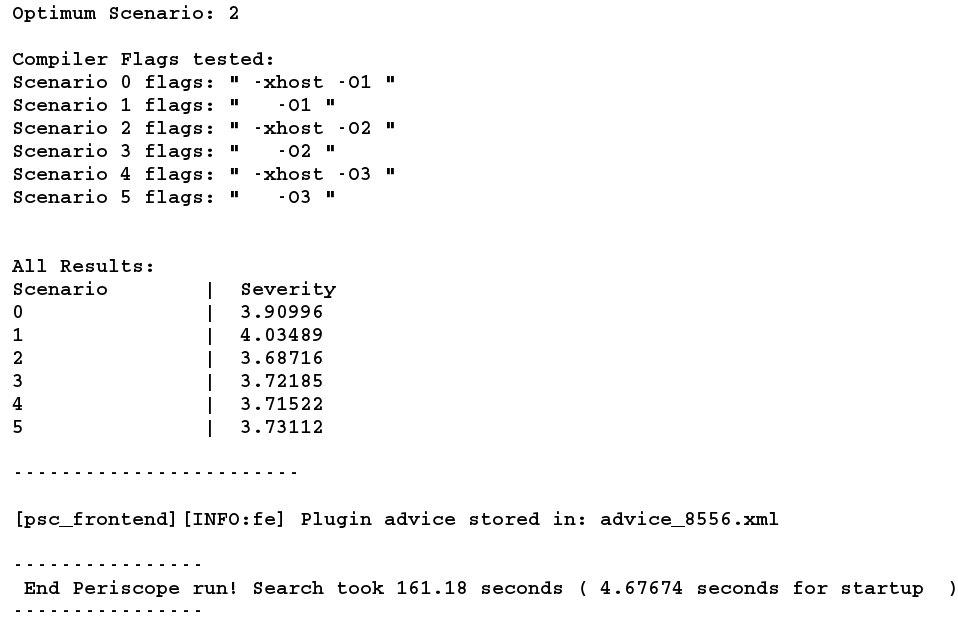
\includegraphics[width=\textwidth]{../BPG/images/uc1_fast_interactive.png}
	\caption{Sample output for the BT-MZ appliation showing the reduction in time spent in initialization of PTF by using the FastInteractive flag.}
	\label{fig:uc1_fast_interactive}
\end{figure}

\subsection{Manual instrumentation}
Manual instrumentation is an important technique to be exploited when dealing with codes that use complex language constructs and that are consequently difficult to instrument using the built-in {\tt psc\_instrument} command (it is often useful for C++ codes). In our second use case we will manually instrument a C++ application and run it using the CFS plugin. The following subsections will walk through each step involved in the manual instrumentation of the code and its significance. We instrument code in order to inform PTF about computationally intensive parts of a given code so as to steer the focus of PTF  tuning efforts. These steps mainly involve identifying the computationally intensive parts of the code through profiling, and then marking them with specific PTF library calls . The build procedure is subsequently updated to link against the PTF libraries to make these functions available. Finally, a {\tt SIR} file is created to convey manual instrumentation information to PTF.

\subsubsection{Application background}
By way of demonstrating best practices on manual instrumentation we will focus on the C++ LULESH (\textbf{L}ivermore \textbf{U}nstructured \textbf{L}agrangian \textbf{E}xplicit \textbf{S}hock \textbf{H}ydrodynamics) \cite{LULESH} code. LULESH is one of the proxy applications proposed by Lawrence Livermore National Lab (LLNL) as part of co-design efforts to address exascale challenges. By its nature, LULESH is a highly simplified application, hard-coded to only solve a simple Sedov blast problem with analytic answers. It represents the numerical algorithms, data motion, and programming style typical in HPC applications written in C or C++.

\subsubsection{Finding the phase region}

To identify the computationally intensive parts of LULESH we will profile the code using gprof by adding the {\tt -pg} compiler flag. This requires updating the Makefile of the application. After executing the newly compiled binary we obtain the profiling data in the form of a binary file named {\tt gmon.out}. Using a tool such {\tt gprof} allows us see the amount of time spent in each function of our application. Figure \ref{fig:uc3_gprof_output} shows partial output from the gprof profile of LULESH running in sequential mode, showing that the majority of time during execution was spent in the {\tt LagrangeLeapFrog} function.
	
\begin{figure}[H]
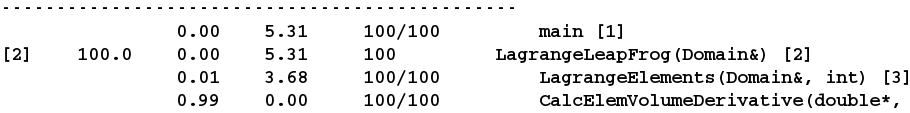
\includegraphics[width=\textwidth]{../BPG/images/uc3_gprof_output.png}
\caption{Partial output from {\tt gprof} showing hotspot functions in LULESH.}
\label{fig:uc3_gprof_output}
\end{figure}
	
Inspecting the source code reveals that the {\tt LagrangeLeapFrog} function is called within an iterative time-stepping loop (a so-called`` phase region"). Figure \ref{fig:uc3_timestep_loop} shows a segment of LULESH source code from the {\tt lulesh.cc} file, containing the while loop which iterates over a given number of time-steps.

\begin{figure}[H]
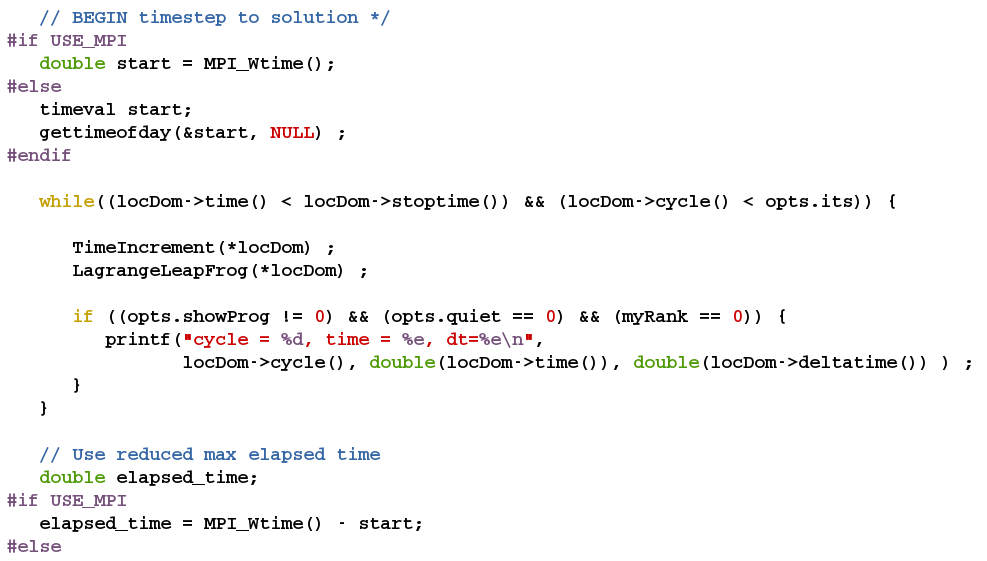
\includegraphics[width=\textwidth]{../BPG/images/uc3_timestep_loop.png}
\caption{The compute intensive while loop interating over the timesteps and calling the {\tt LagrangeLeapFrog} function in LULESH.}
\label{fig:uc3_timestep_loop}
\end{figure}
	
At this stage, we will convey this information about the computationally intensive part of the code to PTF by placing the user region around this segment of the code.
	
\subsubsection{Marking the PTF region in the source code}

To start with the instrumentation we need to mark the beginning and end of the application. Figure \ref{fig:uc3_start_main_region} shows how we mark the beginning of an application using the PTF region, and Figure \ref{fig:uc3_end_main_region} shows the end of PTF region.

The following guidelines need to be followed when marking the start of a PTF region in the example code we work with here (LULESH):
		
\begin{itemize}
	\item Firstly, we have to include a header file {\tt mrimonitor.h}.

	\item Then we need to find the {\tt main} function of the application and declare some of PTF-specific variables.

	\item Next we call the {\tt startMonLib()} function to start a monitoring library.

	\item We then insert a call to the {\tt startRegion()} function with the third argument as the line number where the call to start a monitoring library is made.

	\item Finally, we put the content of the entire {\tt main} function into the code block surrounded by the curly braces.
\end{itemize}
	
	\begin{figure} [H]
		\centering
		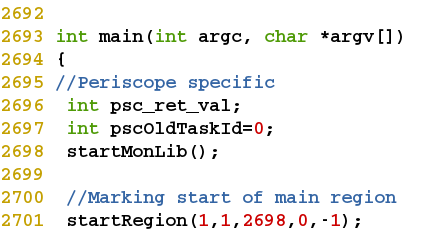
\includegraphics[scale=0.75]{../BPG/images/uc3_start_main_region.png}
		\caption{The {\tt main} function is marked with the start of a PTF region.}
		\label{fig:uc3_start_main_region}

	\end{figure}
	
		The following guidelines need to be followed while marking the end of a PTF region.
		\begin{itemize}
			\item Assign a zero value to {\tt psc\_ret\_val} variable.
			\item Make a call to {\tt endRegion()} function with the same arguments as that of the {\tt startRegion()} function.
			\item Stop the monitoring library by calling {\tt stopMonLib()} function.
			\item Place these calls before the {\tt MPI\_Finalize()} call.
		\end{itemize}

	\begin{figure}[H]
		\centering
		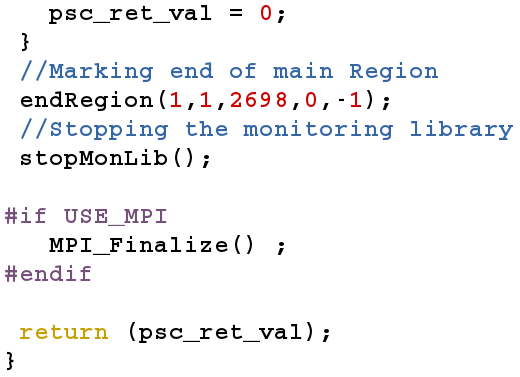
\includegraphics[scale=0.6]{../BPG/images/uc3_end_main_region.png}
		\caption{The end of the PTF region is marked with in the {\tt main} function.}
		\label{fig:uc3_end_main_region}		
	\end{figure}

\subsubsection{Marking a user region in the source code }

A user region can be used to mark the phase region of the application. It then identifies a part of the code where we want PTF to focus it's optimization efforts. User region pragmas are placed around computationally intensive code sections. In the case of a computationally intensive loop traversing a high trip count, performance of a single iteration of the loop for a particular optimization can often be representive of the overall performance of an application for that optimization. When such a loop is marked as a User Region, PTF executes the loop for only a single iteration to measure the performance improvements.
	
	\begin{figure}[H]
		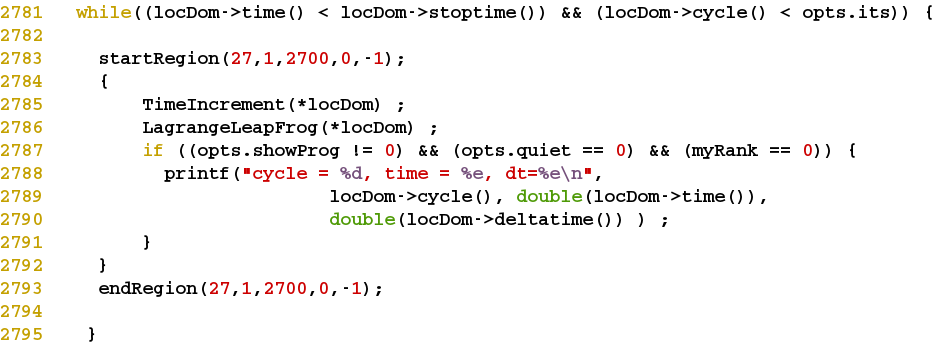
\includegraphics[width=\textwidth]{../BPG/images/uc3_instrumented_loop.png}
		\caption{Instrumented version of the timestep loop.}
		\label{fig:uc3_instrumented_loop}
	\end{figure}

Figure \ref{fig:uc3_instrumented_loop} shows the updated time-stepping loop. The following guidelines need to be followed when marking code with a user region.
	
	\begin{itemize}
		\item Call {\tt startRegion()} and {\tt endRegion()} functions at the beginning and end of the loop. Make a note that both the function calls are inside the loop.
		\item The third parameter in the function is the line number of the statement before the outer {\tt startRegion()} call.
		\item The user region marking the phase region entails a collective synchronization. PTF configures application monitoring in {\tt startRegion()} and {\tt endRegion()}. This configuration leads to a barrier synchronization. 
	\end{itemize}
	
\subsubsection{Updating makefile to link against PTF libraries}

When instrumenting the code we include the {\tt mrimonitor.h} header file and insert function calls {\tt startRegion} and {\tt endRegion()} to mark the region to be instrumented. While compiling this manually instrumented code we need to inform the compiler about the location of the header file to include it, and also inform the linker about the name and location of the libraries containing the necessary function calls.
	
	\begin{figure}[H]
		\centering
		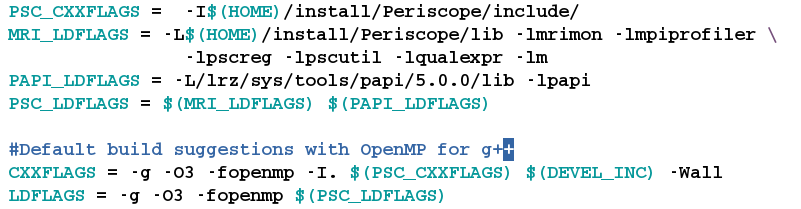
\includegraphics[scale=.65]{../BPG/images/uc3_makefile.png}
		\caption{Updated {\tt Makefile} to find PTF header files and link the PTF libraries.}
		\label{fig:uc3_makefile}
	\end{figure}
	

In Figure \ref{fig:uc3_makefile} we show an updated {\tt Makefile} for LULESH. Relevant changes include -
	
	\begin{itemize}
		\item The path for the PTF headers is provided to compiler by adding to {\tt CXXFLAGS}.
		\item The path and name of the PTF libraries are provided using {\tt LDFLAGS} variable.
		\item Additional libraries  are pointed to by aggregating them into the {\tt PSC\_LDFLAGS} variable.
	\end{itemize}
	
	\subsubsection{Generating a {\tt SIR} File}
	
By way of a {\tt SIR} file we can inform PTF about the outer and User Regions generated during the manual or automatic instrumentation, with an example {\tt SIR} file shown in Figure~\ref{fig:uc3_sir_file} .
	
	\begin{figure}[H]
		\centering
		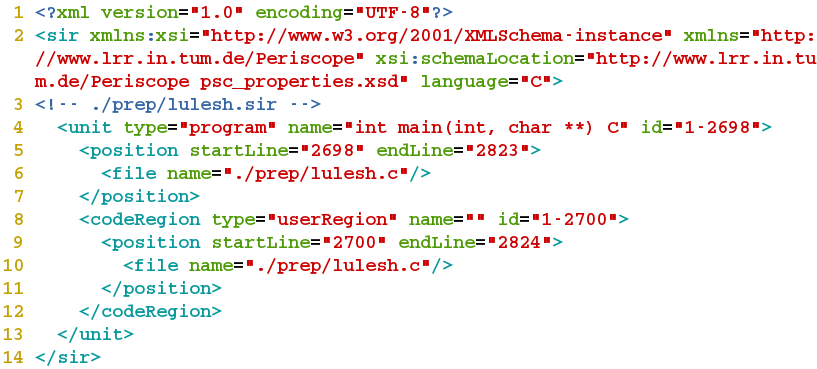
\includegraphics[scale=.65]{../BPG/images/uc3_sir_file.png}
		\caption{{\tt SIR} file}
		\label{fig:uc3_sir_file}
	\end{figure}
	
To generate a {\tt SIR} file one can follow template or any existing {\tt SIR} file and update it using the guidelines below to suit a given application.

\begin{itemize}

\item Update the {\tt id} field of a unit tag, to 1-(line number of a line where the call to {\tt startMonLib()} is made). The id of a region is composed of the two numbers, you can choose both but unique.

\item The {\tt position} tag under the unit tag should contain {\tt startLine} as a line number specified in the outer tag after 1  and {\tt endLine} should be the line where the outer region ends.

\item The {\tt file} tag should contain the value {\tt name} in the {\tt ./\textless file\_name\textgreater.c}.  The name of the file containing the outer region should go here.

\item The {\tt codeRegion} should have {\tt id} as 1-(line number of a line where the call to {\tt startRegion()} is made) and {\tt type} should be {\tt userRegion}.

\item The {\tt position} and {\tt file} tag should follow the same format as the {\tt position} tag used above.
		
		
\end{itemize}	
	
\subsubsection{Executing the instrumented application with PTF}

Once the instrumentation is completed, the execution of the application is carried out in the same way as of an application automatically instrumented with the {\tt psc\_instrument} command. In this case, we use the following commands:

\begin{verbatim}
      module load gcc ace/6.1 papi
      module load boost/1.45 gcc mpi.intel
      
      psc_frontend --apprun="./lulesh2.0" --sir="./lulesh.sir"
                   --mpinumprocs=8 --tune=compilerflags
\end{verbatim}

The \texttt{module load} commands configure an environment on the SuperMUC system with paths for the necessary libraries and the \texttt{psc\_frontend} command is used to start the tuning running the CFS plugin. Here, we have used the same configuration file {\tt cfs\_config.cfg} as that used for the BT-MZ use case.
		
	
\subsubsection{Improving the accuracy of PTF results}
In the case of an instrumented applications with a single iteration of a computationally intensive loop executing for a short amount of time, tuning results may not be consistent. This is mainly due to OS noise or the resolution of the instrumentation. In such cases we can modify the code by increasing the number of iterations to be instrumented in order to obtain consistent results. This can also be achieved by loop splitting. Figure \ref{fig:lulesh_split_loop.png} shows the version of LULESH code shown in Figure\ref{fig:uc3_instrumented_loop} after splitting the loop into two loops. In the new version, a user region is placed around the inner loop which runs for 1000 iterations.

\begin{figure}[H]
	\centering
	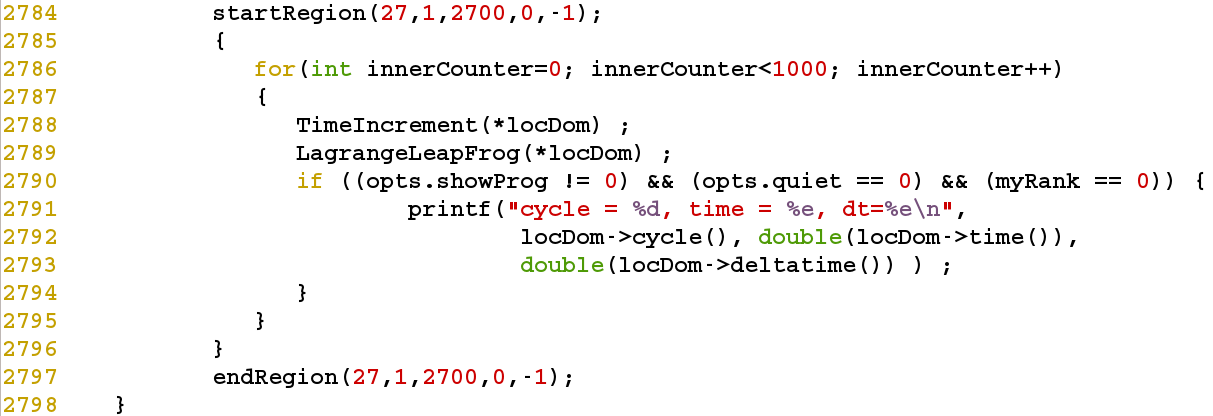
\includegraphics[width=\textwidth]{../BPG/images/lulesh_split_loop.png}
	\caption{Splitting the loop to execute more iterations in the User Region in LULESH.}
	\label{fig:lulesh_split_loop.png}
\end{figure}

\subsubsection{Results for LULESH}
	\begin{itemize}
	\item \textbf{CFS Plugin}

Figure \ref{fig:uc3_cfs_results_exec_time} demonstrates that the combination of the compiler flags suggested by PTF results in ~9.5\% improvement in the overall execution time of LULESH.
	
	\begin{figure}[H]
	\centering
	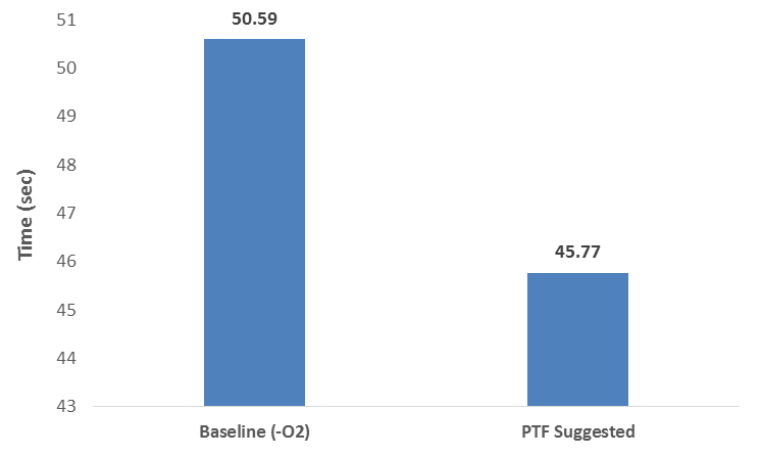
\includegraphics[scale=.60]{../BPG/images/uc3_cfs_results_exec_time.png}
	\caption{Execution time with the optimal compiler flags suggested by PTF and the baseline reading taken without using PTF.}
	\label{fig:uc3_cfs_results_exec_time}
\end{figure}
	\end{itemize}

\subsubsection{Additional tips}
\begin{itemize}

\item It is recommended to add a delay of one or more executions of the phase region in the {\tt psc\_frontend} command using the {\tt --delay} flag to avoid the warm up phase of the application.

\item Check the reproducibility of the measurements.

\end{itemize}
